\begin{frame}
  \frametitle{\problemtitle}
  \begin{block}{Problem}
    Given some dice with various numbers of sides, output the possible sums of dice rolls in order of probability.
  \end{block}
  \pause
  \begin{block}{Solution}
    \begin{itemize}
      \item Use dynamic programming, adding the dice one by one to the current probability distribution.
      \item If the current distribution is $\pi$ and we add a $k$-sided die, then the new distribution $\pi'$ is
        \[ \pi'(n) = \frac{1}{k}(\pi(n-1) + \dots + \pi(n-k)). \]
      \item \emph{Pitfall}: beware of integer overflow when using counts instead of probabilities.
    \end{itemize}
  \end{block}
\end{frame}
\begin{frame}
  \frametitle{\problemtitle}
  \begin{block}{Easier Solution}
    \begin{itemize}
      \item Notice that the probability distribution is always symmetrical, e.g.\ for two d4 and one d6:
        \begin{center}
          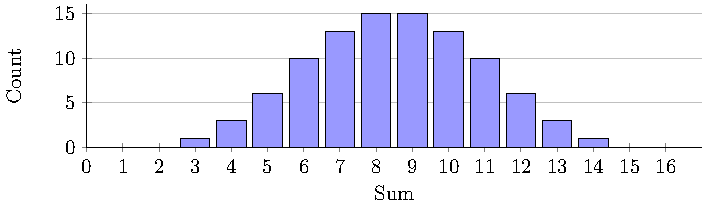
\includegraphics[width=0.6\textwidth]{histogram}
        \end{center}
      \item This means we can find the final order without computing any probabilities!
      \item The solution is easiest to construct by starting at the extremes and taking turns moving inwards.
    \end{itemize}
  \end{block}
\end{frame}
